\nnarticleheader{Plato and the Philosophical Value of Geometry}{Mickey Fairorth, Haverford '19, St. Charles Borromeo Seminary}
“Let no one ignorant of geometry enter here.” These words, engraved above the doorway, greeted any Athenian bold enough to venture into Plato’s Academy. As a student of Socrates, Plato is known to the world as one of the essential Greek philosophers and as one of the greatest thinkers ever. Whereas Socrates wrote nothing down, choosing instead to dialogue with others, Plato left society with an extensive body of work. Besides transcribing Socrates’ wisdom for the world to access, Plato established his Academy in 387 B.C. for eager minds to discuss philosophy. As a school of abstract thought, the engraving above the doorway begs us to question why Plato insisted his students know geometry before entering the Academy.

Part of the reason Plato demanded a knowledge of geometry was because he himself contributed to this field and found it integral to understanding the world. In particular, Plato believed that the raw elements of the universe were composed of regular, convex polyhedrons. These objects, known as Platonic Solids, have congruent, regular, polygonal faces with an equal number of faces meeting at every vertex. In simpler terms, each face is a regular shape (equilateral triangle, square…), and each face is identical. Only five solids meet these criteria:

\begin{center}
The tetrahedron: four equilateral triangular faces.\\
The cube: six square faces.\\
The octahedron: eight equilateral triangular faces.\\
The dodecahedron: twelve pentagonal faces.\\
The icosahedron: twenty equilateral triangular faces.\\
\end{center}

\begin{figure}[h]
  \begin{center}
    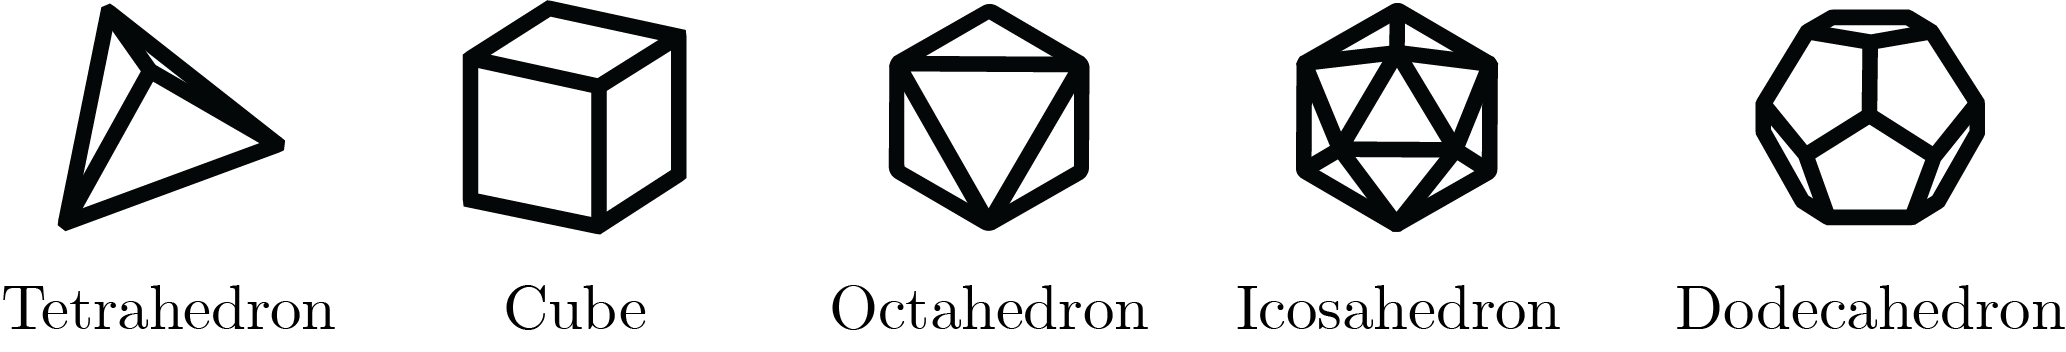
\includegraphics[scale=.925]{fairorth_platonic_solids.png}
  \end{center}
\end{figure}

While Plato’s conception that the universe is composed of these solids is certainly flawed, he properly emphasized the importance of geometry in understanding the world around us. Thus, before someone could enter his Academy in search of life’s toughest truths, it was fitting to have a basic understanding of the space in which they lived. 
	
More importantly, however, Plato needed his students to grasp geometry because it demonstrated an ability to think clearly. Geometry is built entirely upon axioms, deductions from axioms, and further deductions from simpler conclusions. Axioms, derived from the Greek word axios which means “worthy,” are fundamental statements that cannot and need not be proven. Euclid, the father of Euclidean Geometry, exemplifies axioms perfectly in providing such definitions as, “the angles of a triangle always add up to 180 degrees.” Also called postulates, these axioms are generally obvious and self-evident. From basic axioms, mathematicians have derived theorems, which combine axioms in a logically sound manner to find more specific and helpful geometric rules. One of the most famous theorems is the Pythagorean Theorem ($a^2 + b^2 = c^2$) which can provide the length of a side of a right triangle given the other two sides’ lengths. Mathematicians can also use proven theorems as starting points for further conclusions. 

While it is true that Plato investigated geometry and found it useful in itself, he desired the principles of thought behind the math more than the math alone; Plato was not looking to assemble an academy of mathematicians to prove spatial theorems but rather a collection of thinkers who could reason from one thought to the next. Despite the differences in subject matter, philosophy is built on the exact same principles as geometry. From axioms, such as “good is to be sought and evil is to be avoided,” philosophers deductively reason to other conclusions. For instance, one might assess that stealing is evil, and since evil is to be avoided, stealing must be avoided as well. While simple, in theory, these logical syllogisms become increasingly complicated and difficult to evaluate as they move further away from the axioms. Hence, it is imperative for a thinker to see clearly how one premise moves to the next and how any conclusion relates back to the principles upon which it is founded. 

At the end of the day, Plato is not known as a mathematician; he is a philosopher. However, as a philosopher, he saw the beauty and value of geometry that is often missed in high-school classrooms. In the real world, it is not essential to know the Side-Angle-Side Theorem. Yet, for anyone who wishes to impact those around them, it is necessary to think clearly, to reason from a principle to a conclusion, and to employ logical deduction. Above Plato’s Academy of philosophy stood the words “Let no one ignorant of geometry enter here.” If someday, by some odd chance, I become a geometry teacher, my students will read these words as they exit each day from class: “Let no one ignorant of philosophy exit here.”\\\\

\begin{figure}[h]
  \begin{center}
    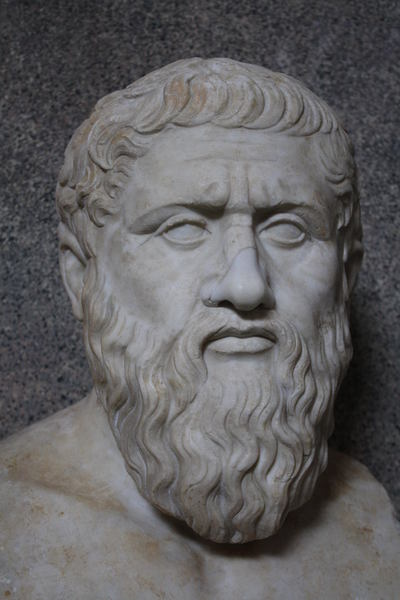
\includegraphics[scale=.75]{fairorth_plato.jpg}
  \end{center}
  \caption{A bust of Plato, 428/427 or 424/423 – 348/347 BCE.}
\end{figure}
